\documentclass[dvipdfmx]{article}
\usepackage[dvipdfmx]{graphicx}
\usepackage{amsmath, amssymb}
\usepackage{mathtools}
\usepackage{here}
\begin{document}
\title{Weekly Report}
\author{Riku Gondow}
\maketitle
\section{Progress}
\begin{itemize}
    \item Finish implementing Openmax (Since the accuracy is expected to be almost the same on a clean dataset, I thought about preprocessing methods first.)
    \item Check Preprocessing code shared by Kitagawa-San
    \item Survey preprocessing method for radar signal
\end{itemize}


\section{Keio Hospital Dataset}
I checked the Keio Hospital Dataset and applied BPF [0.6-2.0 Hz]. The results are shown below.

\begin{figure}[H]
\begin{center}
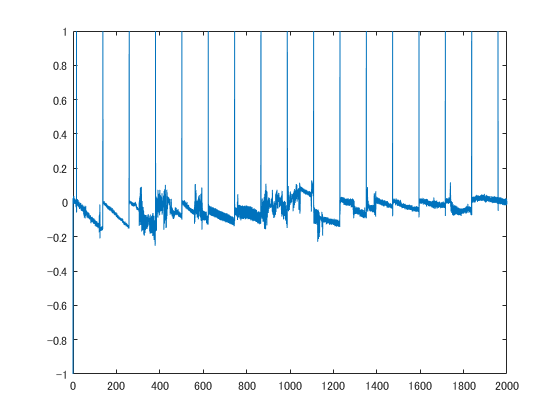
\includegraphics[width=0.8\linewidth]{"./img/nonfiltered.png"}
\end{center}
\caption{Raw signal}
\end{figure}

\begin{figure}[H]
\begin{center}
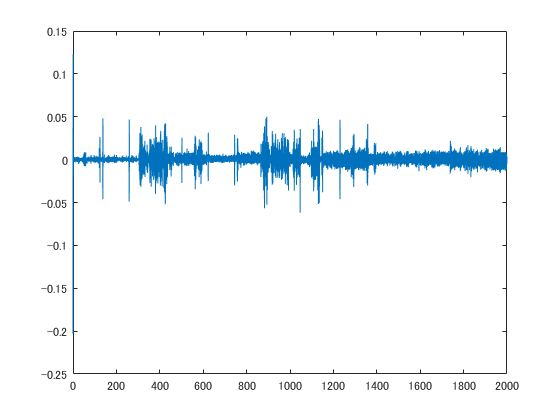
\includegraphics[width=0.8\linewidth]{"./img/filtered.png"}
\end{center}
\caption{Filtered signal}
\end{figure}

Most of the jumps that appeared in the raw signal have disappeared.

\section{Survey: Preprocessing method}
I found sevral methods that seem to work for noisy dataset.
\begin{itemize}
    \item Adaptive noise cancellation methods
    \begin{itemize}
        \item NLMS(Normalized Least Mean Square)
        NLMS has fast convergence as compared with the conventional LMS algorithm, but has a drawback of increased misadjustment.
        \item TDLMS(Transform domain Least Mean Square)
        Transform domain LMS algorithms is a class of robust preconditioned algorithms having good tracking capabilities in non stationary environments. Application of an orthogonal transform, followed by a power normalization step, has the ability to reduce the eigenvalue spread of input correlation matrix, which results in an increase of convergence speed of the algorithm.
    \end{itemize}
    
    \begin{figure}[H]
    \begin{center}
    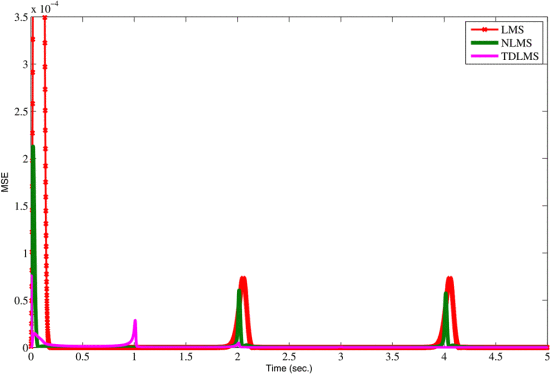
\includegraphics[width=\linewidth]{"./img/LMS_comp.png"}
    \end{center}
    \caption{Comparison of LMS methods applied for ECG}
    \end{figure}

    \item Non-Local Means of Denoising Techniques

    Non-local Means of Denoising (NLM):Non-local means of denoising was used as an image denoising technique.
    The signal regions near to the high amplitude regions but not a part of it are less averaged than it need to be.
    Combining the advantages of NLM with Discrete Wavelet Transform (DWT) a filtering on ECG is presented in [2]. This work involves grouping similar sample blocks to form a matrix called Similarity Data Matrix (SDM) as a measure of similarity between the blocks and then performing DWT coefficient shrinkage to remove noise. The technique is found to be far better than NLM and EMD-Wavelet based denoising methods.
    Figure 2 shows that NLWT is able to remove noise while retaining high-frequency features.

    \begin{figure}[H]
    \begin{center}
    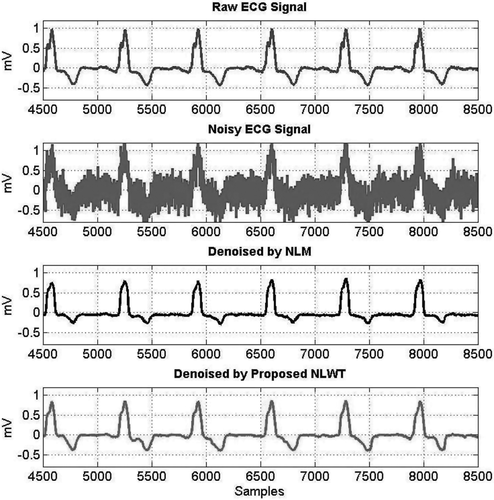
\includegraphics[width=\linewidth]{"./img/NLM_comp.png"}
    \end{center}
    \caption{ECG before and after NLM or NLWT}
    \end{figure}

    \item EEMD(Ensemble Empirical mode decomposition)

    Ensemble EMD (EEMD) is a new noise assisted data analysis method (NADA) proposed by Z. Wu and N. E. Huang [3] to overcome the scale separation problem in EMD. EEMD defines the true IMF components as the mean of an ensemble of trials. Since the noise in each trial is different in separate trials, it is canceled out in the ensemble mean of enough trials.

    \item Variational Mode decomposition

    Variational Mode decomposition followed by discrete wavelet transform and constrained least squires (VMD-DWT-CLS) is proposed in [4].
    VMD is used for optimal reconstruction of the original input signal by decomposing the input signal into sum of variational mode functions (VMFs). Daubechies Wavelet coefficient shrinkage Threshold is selected based on SURE method. Comparative study between EMD-DWT-CLS, VMD-DWTCLS and its various combinations for ECG noisy input signal is presented the paper. Varying AWGN variance value in the signal for different Decomposition levels, SNR and MSE are evaluated. Results show that VMD-DWT-CLS is the best amongst them.

    \begin{figure}[H]
    \begin{center}
    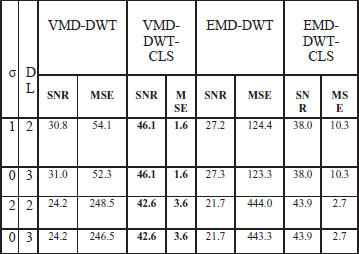
\includegraphics[width=0.85\linewidth]{"./img/VMD_comp.png"}
    \end{center}
    \caption{Performance evaluation of VMD-DWT, VMD-DWT-CLS, EMD-DWT and EMD-DWT-CLS denoising techniques}
    \end{figure}
\end{itemize}

\section{Next Plan}
\begin{itemize}
    \item Prepare dataset (keio Hospital Dataset or new one)
    \item Confirm accuracy for noisy dataset
    \item Brush up the methods for noisy dataset (e.g., change the classifier to openmax, adopt a denoising method other than BPF, etc.)
\end{itemize}

\begin{thebibliography}{99}
\bibitem Haritha, C., M. Ganesan, and E. P. Sumesh. "A survey on modern trends in ECG noise removal techniques." 2016 International Conference on Circuit, Power and Computing Technologies (ICCPCT). IEEE, 2016.
\bibitem Yadav, Santosh Kumar, Rohit Sinha, and Prabin Kumar Bora. "Electrocardiogram signal denoising using non‐local wavelet transform domain filtering." IET Signal Processing 9.1 (2015): 88-96.
\bibitem Gaikwad, Kaustubh Manik, and Mahesh Shrikant Chavan. "Removal of high frequency noise from ECG signal using digital IIR butterworth filter." 2014 IEEE Global Conference on Wireless Computing \& Networking (GCWCN). IEEE, 2014.
\bibitem Lahmiri, Salim, and Mounir Boukadoum. "Physiological signal denoising with variational mode decomposition and weighted reconstruction after DWT thresholding." 2015 IEEE international symposium on circuits and systems (ISCAS). IEEE, 2015.
\end{thebibliography}
\end{document}